\tikzset{thick,every node/.style={scale=1}}
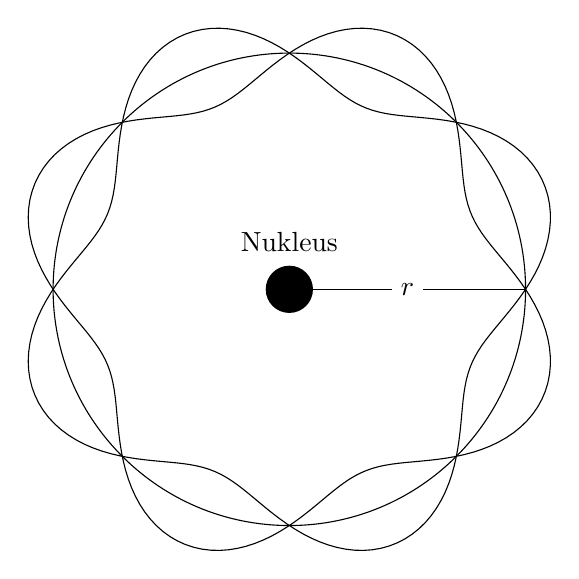
\begin{tikzpicture}
  \def\nucRad{0.3};
  \def\cirRad{3};
  \def\sinAmp{1};
  \def\sinPer{2};

  \fill (0,0) circle(\nucRad);
  \node at (0,2*\nucRad) {Nukleus};
  \draw (0,0) circle(\cirRad);
  \draw[domain=0:360,samples=200] plot (\x:{\cirRad-\sinAmp/2+\sinAmp*(sin((\x-22.5)*\sinPer))^2});
  \draw[domain=0:360,samples=200] plot (\x:{\cirRad-\sinAmp/2+\sinAmp*(sin((\x+22.5)*\sinPer))^2});
  \draw (0,0) to node[pos=0.5,fill=white] {$r$} (\cirRad,0);

\end{tikzpicture}
